\documentclass[journal, a4paper,11pt]{IEEEtran}

\usepackage{graphicx}

%\usepackage{subfigure} 
\usepackage{setspace}

\usepackage{url}    
%\usepackage{stfloats} 

\usepackage{amsmath}    

\usepackage{ragged2e}
\usepackage{graphicx}

\linespread{1.3}

\usepackage[nocompress]{cite}

\def\citepunct{,\,}

\begin{document}

\begin{titlepage}
	\centering
    \vspace{2cm}
    {\scshape\LARGE\bfseries Physics Studies for a Very High \par Energy Electron-Proton Collider\par}
    \vspace{2cm}
	{\scshape\Large\bfseries Literature Review\par}
	\vspace{2cm}
	{\Large Pranav Rao\par}
	\vspace{2cm}
	{\scshape\Large Department of Physics and Astrophysics\par University College London\par}
	\vspace{3cm}
	{\huge\bfseries\par}
	{\large First Supervisor : Prof. Matthew Wing\par Second Supervisor: Prof. Alessio Serafini\par}
	\vspace{6cm}
	Word Count: 1788

	\vfill
\end{titlepage}

\justify

\begin{abstract}
This literature study aims to provide context and motivation for the project that is being undertaken. It explores the subjects of deep inelastic scattering, plasma wakefield acceleration and a very high energy electron proton collider. 
\end{abstract}

\section{Introduction}

The main limitation of how well the structure of the proton can be understood is the energy with which the proton is probed. This limitation arises from the design of current accelerator technology. A Very High Energy electron Proton collider (VHEeP) is proposed as the next step forward in high energy physics, using a new linear acceleration technique; proton driven plasma wakefield acceleration which is currently in the proof of concept stage. The centre of mass energy scales of the VHEeP will allow for new kinematic scales to be probed.

This literature study contains the background information required to undertake the study of the proposed VHEeP. It also contains the aims and motivations of the project along with a time-line of the major milestones of the project.

\section{Background}

\subsection*{\textbf{Deep Inelastic Scattering}}

Electron-proton collisions at sufficiently high energies result in the proton breaking up into hadrons, this process is referred to as Deep Inelastic Scattering (DIS) shown in Fig.\ref{fig:DIS}. By studying the scattering angles of the electrons the theory of protons being composite particles containing three valance quarks was proved. Elastic scattering, where the proton is not broken up, does occur at high energies as well, DIS is the dominant collision type at high energies.

\begin{figure}[!h]
	\centering
		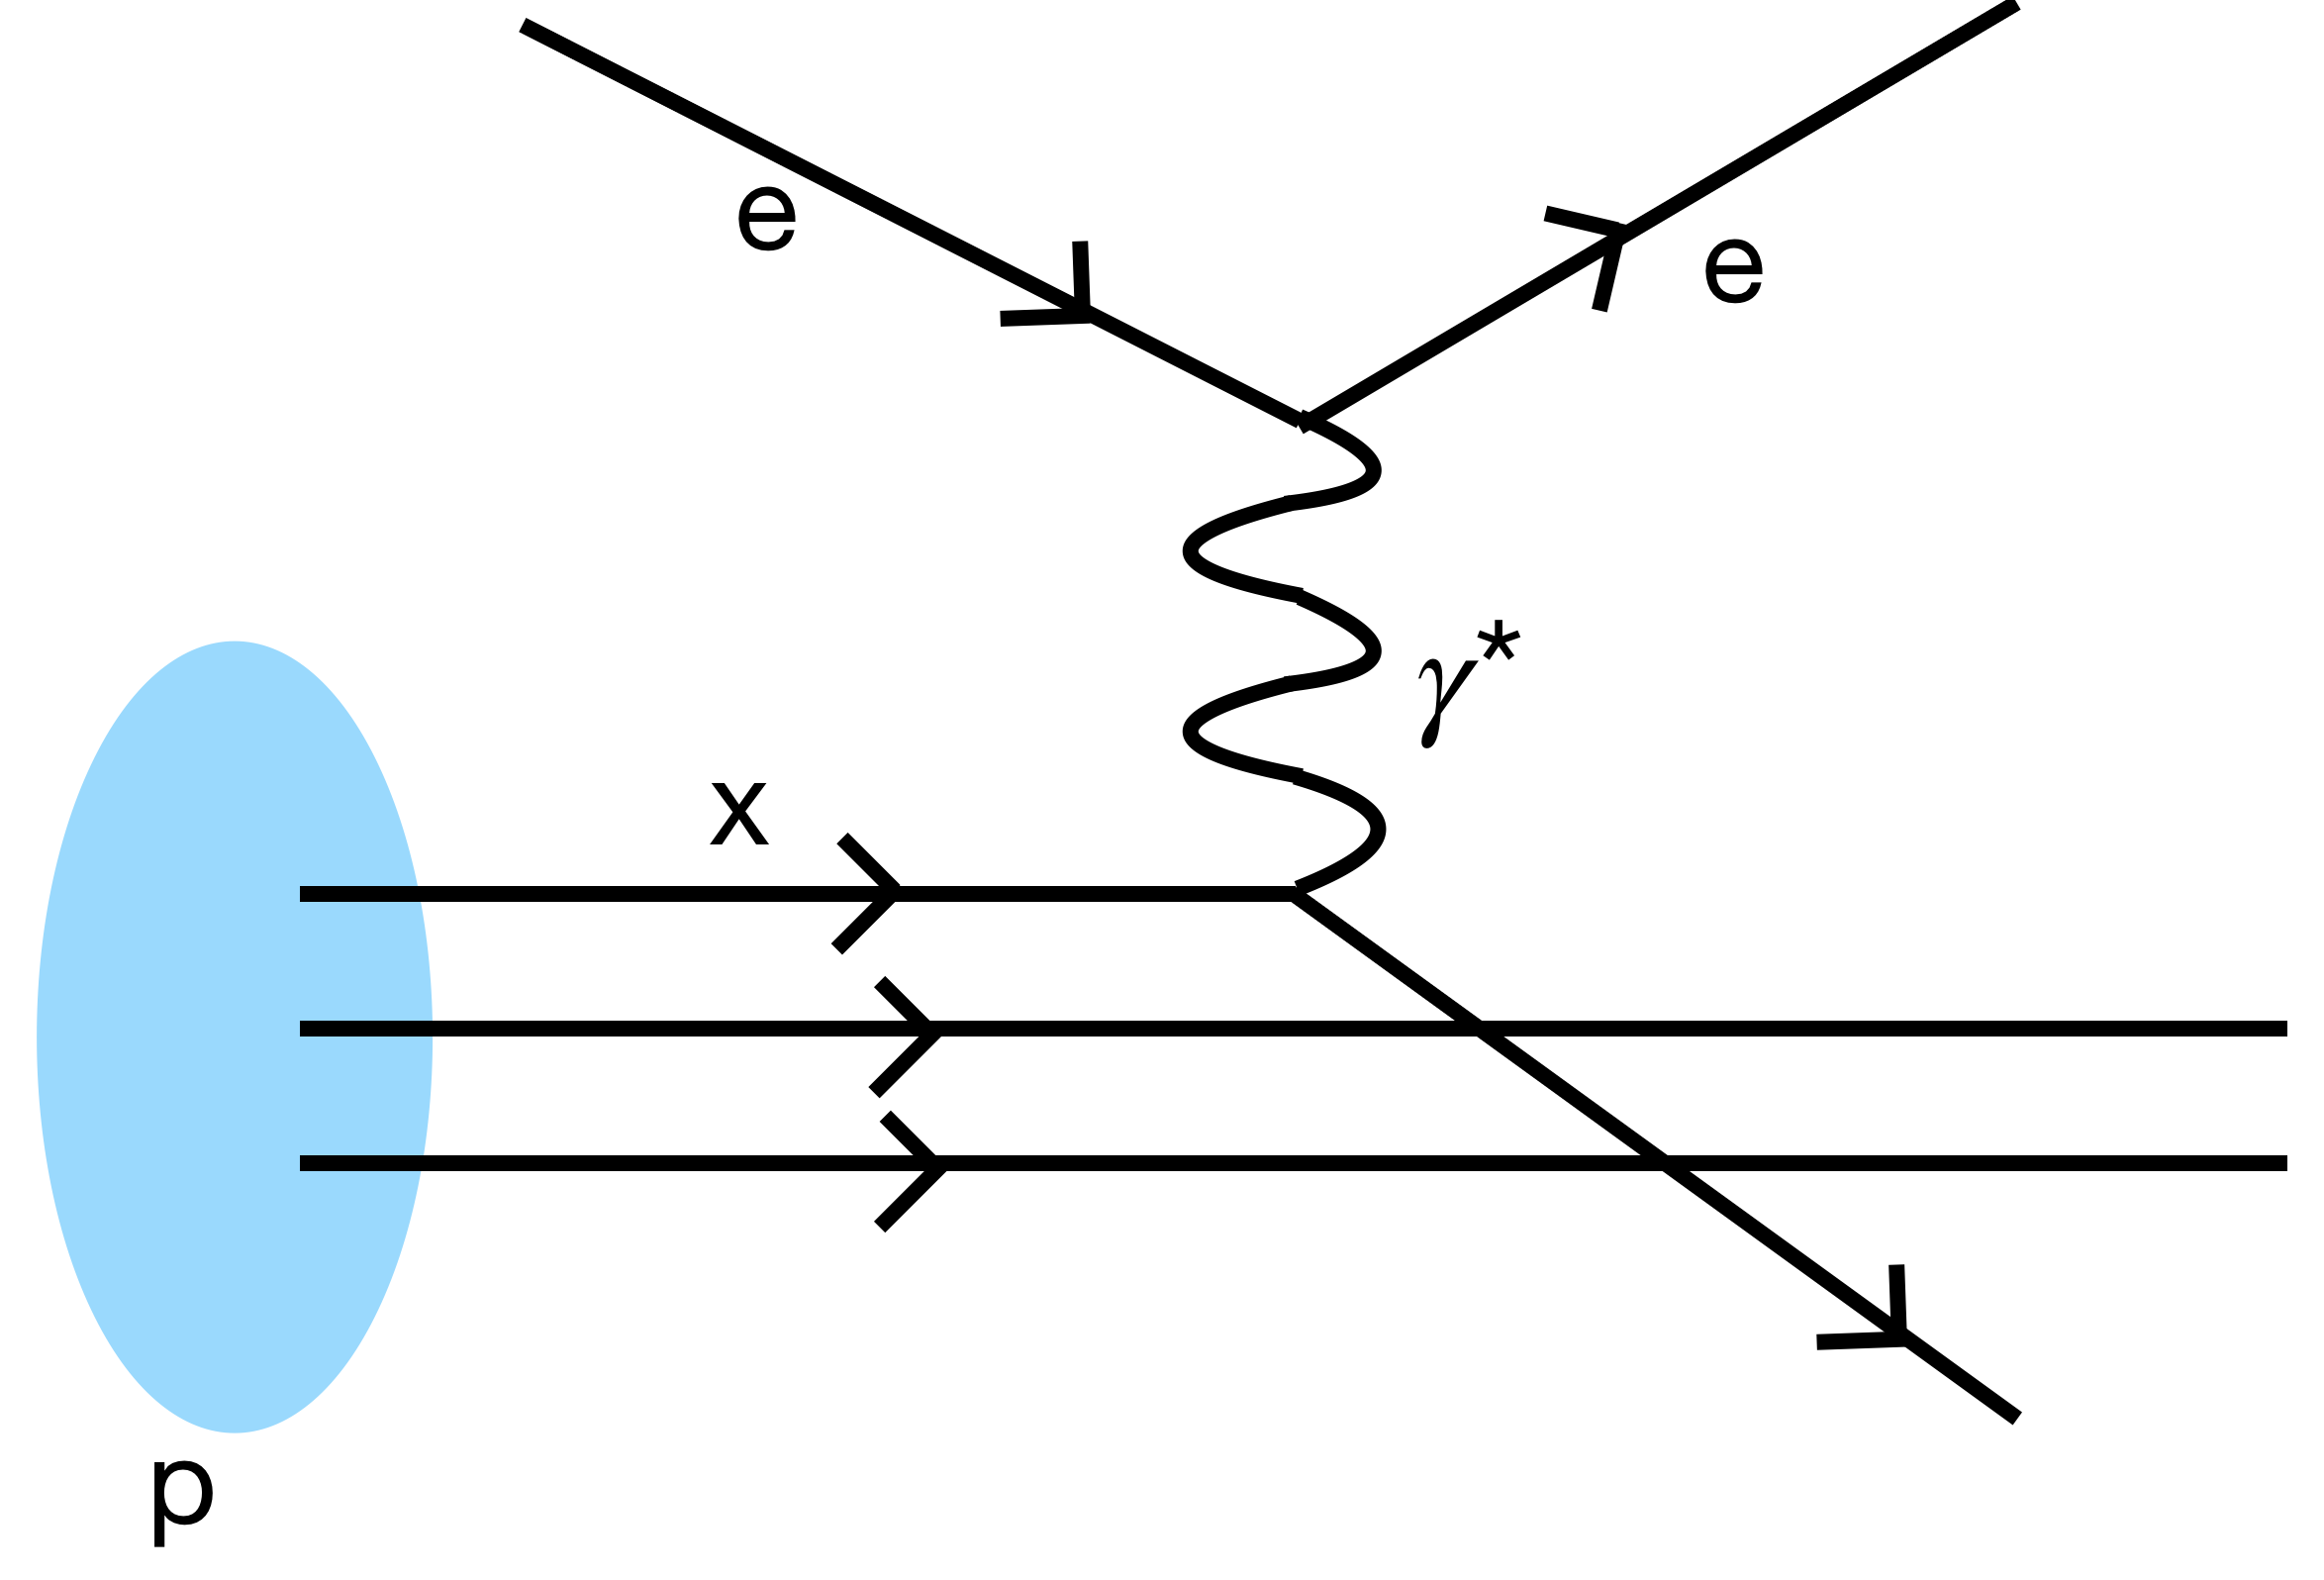
\includegraphics[width =0.45\textwidth]{DIS.png}
		\caption{Schematic diagram showing deep inelastic scattering of an electron and a proton. The electron exchanges a virtual photon $\gamma *$ with one of the valance quarks of the proton and scatters with a difference in momentum $p_1 - p_3$.}
		\label{fig:DIS}
\end{figure}

The hadronic final state consists of many particles and as a result its invariant mass can have a range of values unlike elastic scattering where the invariant mass of the final state is the mass of the proton. This range of values leads to an additional degree of freedom which requires an additional quantity to describe the kinematics of the event. The quantities required are chosen from a list of Lorentz invariant quantities x, y, $\nu$, and $Q^2$. 
The energies at which DIS occurs are high enough to neglect the mass of the electrons while making predictions, as a result a good approximation of $Q^2$ can be made \cite{Modern}:
\begin{equation}
	Q^2 = 4E_1E_3 \sin ^2\frac{\theta}{2}
	\label{eq:Q2}
\end{equation}
which is always positive. In eq (\ref{eq:Q2}), $Q^2$ is the four-momentum squared, $E_1$ is the energy of the incoming electron, $E_3$ is the energy of the scattered electron and $\theta$ is the angle by which the electron is scattered.

Bjorken $x$ is one of the Lorentz invariant quantities that can be used to describe kinematics of DIS. It is given by the following equation \cite{Modern}: 
\begin{equation}
	x = \frac{Q^2}{Q^2 + W^2 - m_p^2}
	\label{eq:x}
\end{equation}
where $W^2$ is the invariant mass of the final hadronic state, and $m_p^2$ is the rest mass of the proton squared. $W^2 \geq m_p^2$ because for baryon number to be conserved, the hadronic state must contain at least one baryon and the proton is the lightest baryon. $W^2 \geq m_p^2$ along with $Q^2 \geq 0$ defines the range of $x$ $0 \leq x \leq 1$. Bjorken $x$ is a variable that describes the elasticity of the scattering process, and when $x = 1$ the scattering process is elastic and $Q^2 = W^2$.

Another Lorentz invariant dimensionless quantity used to describe DIS kinematics is the inelasticity $y$ and it is defined as follows \cite{Modern}:
\begin{equation}
	y = 1-\frac{E_3}{E_1}.
	\label{eq:y}
\end{equation}
The inelasticity can also be understood as the fractional loss in electron energy which also has a range $0 \leq y \leq 1$.

In situations where it is more convenient to work with the energy difference rather than the fractional energy lost, the Lorentz invariant quantity $\nu$ is used, and it is described as \cite{Modern}:
\begin{equation}
	\nu = E_1 - E_3,
	\label{eq:nu}
\end{equation}
and can be understood as the absolute energy lost by the electron in the scattering process.
The kinematics of a DIS collision can be described using any combination of $Q^2$, $x$, $y$, and $\nu$ for a fixed centre of mass energy, except for $y$ and $\nu$ because they are not independent of each other.

\subsection*{\textbf{Plasma Wakefield Acceleration}}

Plasma wakefield acceleration is a technique used for linearly accelerating electrons to sufficiently high energies which have not been achieved before. AWAKE \cite{AWAKE1,AWAKE2} is a proof of concept experiment for accelerating electrons to kinematic regions previously unexplored.

The new frontier of particle colliders are thought to be electron-proton colliders with very high centre of mass energies. Radio frequency accelerators can only achieve $100$ MV/m electric fields \cite{1115} and as a result to excite electrons to the TeV scale, linear accelerators would need to be tens of kms long and circular accelerators would need to have a circumference of hundreds of kms. 

Plasmas can support near light speed waves or wakes which can be used for accelerating electrons. These wakes are made of longitudinal and transverse components, the longitudinal component extracts energy from the drivers (protons) and delivers it to the electrons, and the transverse components focuses the electron bunch. The transverse component has a focusing power many orders larger than conventional magnets used for focusing \cite{0114}.

Plasmas are capable of sustaining potential gradients with order of magnitude of $10$ GV/m when traversed by electron bunches \cite{Bl2007} or laser pulses \cite{Mangles2004}. Due to the low stored energy of electron bunches or laser pulses, multiple acceleration stages would be required for electrons to reach very high energies, proton bunches can instead be used to drive the wakefields.   

Proton driven plasma wakefield acceleration could be the next step for particle colliders to advance, however there are challenges that needs to be overcome one of which is the current length of a proton bunch used to drive the wakefield is too long. Plasmas have an oscillating frequency which needs to be met by the driving frequency to achieve resonance. Plasmas which can provide GV/m gradients have a wavelength in the mm scale, while proton bunches are much longer, in the cm scale \cite{0114}.

A possible solution, which is being explored by AWAKE, is self modulating instability (SMI) \cite{255003}, a mechanism by which the driving frequency can be made to match the plasma frequency. SMI splits bunches of protons into micro bunches which reduces the wavelength of the driving proton beam. Under the right conditions the wavelength can be made to exactly equal exactly one plasma wavelength, achieving resonance. Despite SMI being energy inefficient, it is cost effective and relatively simple to execute, as a result it is a good starting point to use in the proof of concept for wakefield acceleration \cite{1115,0114}.

Another challenge of this type of acceleration is the extremely strict requirements on the uniformity of density of the plasma. The paper published by E. {\"O}z and P. Muggli \cite{OZ} studied the required uniformity for Rubidium plasma and concluded that a uniformity of $0.2\%$ or better would be required. This level of uniformity can be achieved by filling a vacuum with a neutral gas and ionising it with a laser.  

In the most recent paper by AWAKE \cite{0918}, the results of successfully accelerating electrons via a proton driven plasma wakefield are shown. Electrons were accelerated up to 2 GeV in 10 m of plasma. This technique has the potential to accelerate electrons to the TeV scale in just a single accelerating stage.

\subsection*{\textbf{HERA Collider and H1 Collaboration}}

HERA (Hadron Elektron RingAnlage) collider was the only electron-proton collider and it ran from 1992-2007 and had a circumference of 6.3 km. It improved the kinematic region of the proton which could be probed, because previous DIS experiments were conducted with a beam of electrons and a stationary target of protons. Electrons were accelerated to $27.5$ GeV and collided with protons that were accelerated to $900$ GeV \cite{Modern} and it operated with a centre of mass energy of $\sqrt{s} = 318$ GeV \cite{1308}.

The H1 collaboration \cite{H1} was one of the experiments that was located at HERA with the other one being ZUES. Ref \cite{H1} presents measurements of jet cross sections in neutral current (NC) DIS for $5.5 \leq Q^2 \leq 80 GeV^2$ with inelasticities $0.2 \leq y \leq 0.6$. A jet is a narrow cone of hadrons which can be studied to reconstruct the hadronic state produced by the scattering. Neutral current DIS is the scattering mode where the virtual particle exchanged is a photon ($\gamma$) or a Z\textsuperscript{0} boson which are both neutrally charged. H1 studied jet production in the Breit frame which always involves at least one strong vertex, which directly probes QCD.

If quarks were composite particles then deviations from the Bjorken scaling would be expected when the wavelength of the virtual photon was comparable to the size of the quark. As the data collected by H1 was consistent with Bjorken scalling, the radius of the quark is predicted to be smaller than $10^{-18}m$ \cite{Modern}.

\subsection*{\textbf{VHEeP}}

The VHEeP \cite{VHEeP} is a electron-proton collider and is proposed to have a 9 TeV centre of mass, which is a factor of 30 greater than the only other electron-proton collider HERA \cite{HERA}. By probing new kinematic regions, VHEeP has the potential to better understand sections of QCD, the structure of the proton as well as search for physics beyond the Standard Model.

High energy electrons needed for the scattering will be accelerated via the linear accelerating technique; proton driven plasma wakefield acceleration, the concept of which is currently being proved by the AWAKE experiment at CERN. The collider will use the existing LHC infrastructure to provide high energy protons which will drive the plasma wakefield as well as collide with the electrons as shown in fig \ref{fig:VHEeP}.

\begin{figure}
\centering
		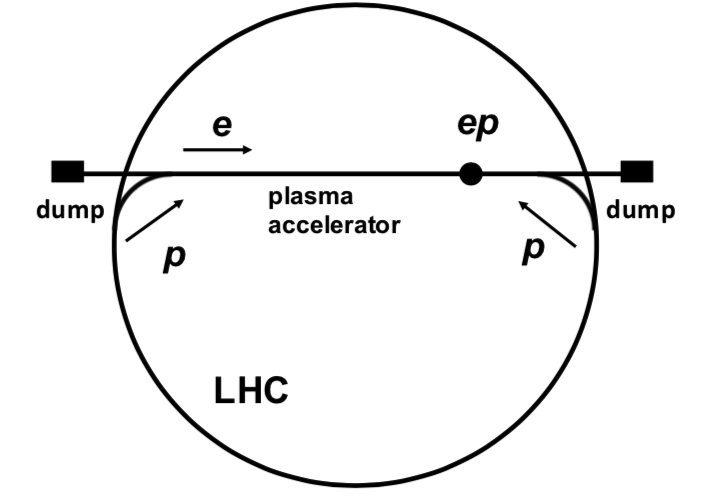
\includegraphics[width =0.45\textwidth]{VHEeP.png}
		\caption{Shows a sketch of the VHEeP using the LHC infrastructure for protons to collide with the electrons and drive the plasma wakefield \cite{VHEeP}.}
		\label{fig:VHEeP}
\end{figure}

\section{Rivet Analysis}

Robust Independent Validation of Experiment and Theory (Rivet) \cite{Rivet} is a class library written in C++ which is used as a method of validating high energy physics Monte Carlo (MC) event generators. It has a host of various analyses, with the capability of writing your own. 

One of the main aims is to write a complete Rivet analysis for the H1 paper \cite{H1}. By writing a Rivet routine it would be possible to validate theory by comparing the data collected by H1 and the MC data generated by Rivet. This can be done using the {\fontfamily{lmtt}\selectfont compare-histos} command in rivet, which accepts multiple AIDA files and compares them with the MC dataset.

The H1 paper contains the parton distribution functions (PDFs) used, the cuts used and the renormalisation scale used by the MC generator. PDFs are momentum distributions of the partons (gluons and quarks) within a proton, cuts are the restrictions on the data selection, and the renormalisation scale affects the value of the strong coupling constant and the PDFs. 

Another aim is to extrapolate the previous analysis of the H1 paper to the TeV scale. This extrapolation could provide an important comparison to the experimental data of very high energy DIS collisions like the collisions that would occur in VHEeP. This analysis will provide a starting point to investigate the expected differences in DIS at the TeV scale. To provide useful comparisons the VHEeP predictive analysis will use similar parameters (cuts, PDFs and renormalisation scales) to the H1 analysis.

Discussions of the predicted behaviour of DIS at different energy scales will be based on the Rivet analysis of the VHEeP and with the use of histograms, compare the two analyses

\section{Timeline}
\noindent The tentative project outline with the key milestones is as shown:
\begin{enumerate}
	\item Background reading and writing the literature study$\sim$ 3 weeks

	\item Importing data and parameters from H1 collaboration into Rivet and writing an analysis $\sim$ 5 weeks

	\item Crosschecking H1 DIS theory using Rivet Analysis and data $\sim$ 8 weeks

	\item Using Rivet Analysis of H1 to make predictions of DIS for VHEeP $\sim$ 7 weeks 

\end{enumerate}

\bibliographystyle{ieeetr}
\bibliography{bib.bib}

\end{document}






